
%(BEGIN_QUESTION)
% Copyright 2006, Tony R. Kuphaldt, released under the Creative Commons Attribution License (v 1.0)
% This means you may do almost anything with this work of mine, so long as you give me proper credit

En samling operasjonsforsterkere kan brukes til å implementere følgende ligning for en proporsjonalregulator, der hver variabel er representert av en likespenning:

$$m = K_p (\hbox{SP} - \hbox{PV}) + b$$

\noindent
Der,

$m$ = Manipulert variabel (utgang)

$K_p$ = Regulatorforsterkning

SP = Settpunkt

PV = Prosessvariabel

$b$ = Bias

\vskip 10pt

$$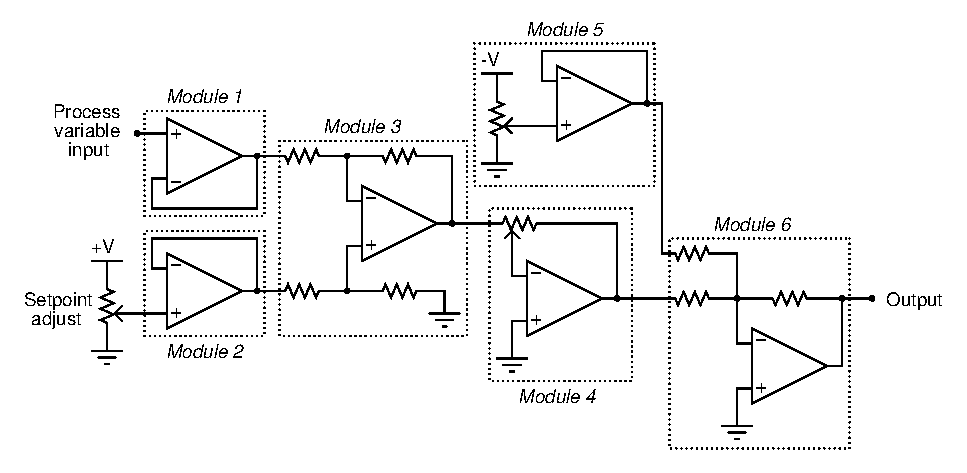
\includegraphics[width=15.5cm]{i01465x01.eps}$$

Identifiser hvilken modul eller hvilke moduler som implementerer hver del av ligningen for proporsjonalregulering.

\begin{itemize}
\item{}Modul 1:
\vskip 5pt
\item{}Modul 2:
\vskip 5pt
\item{}Modul 3:
\vskip 5pt
\item{}Modul 4:
\vskip 5pt
\item{}Modul 5:
\vskip 5pt
\item{}Modul 6:
\end{itemize} 

Angi også om dette er en {\it direktevirkende} eller {\it omvendtvirkende} regulator.
 
\vskip 20pt \vbox{\hrule \hbox{\strut \vrule{} {\bf Forslag til sokratisk diskusjon} \vrule} \hrule}

\begin{itemize}
\item{} Vis hvordan du kan bruke problemløsningsteknikken {\it tankeeksperiment} for å avgjøre om regulatoren er direkte- eller omvendtvirkende.
\item{} Velg tilfeldig en motstand i denne regulatoren og tenk deg at den feiler enten {\it åpen} eller {\it kortsluttet}. Forklar deretter hvordan denne feilen påvirker regulatorens utgangssignal.
\end{itemize}

\underbar{file i01465}
%(END_QUESTION)





%(BEGIN_ANSWER)

\begin{itemize}
\item{}Modul 1: Spenningsfølger (buffer) for PV-signal
\vskip 5pt
\item{}Modul 2: Spenningsfølger (buffer) for SP-signal
\vskip 5pt
\item{}Modul 3: Differensialforsterker (beregner feilsignal)
\vskip 5pt
\item{}Modul 4: Forsterker med variabel gain (multipliserer feilsignal med $K_p$, justert med potensiometer)
\vskip 5pt
\item{}Modul 5: Spenningsfølger (buffer) for bias-signal
\vskip 5pt
\item{}Modul 6: Summeringstrinn som legger bias-signal til utgangen fra forsterkeren
\end{itemize} 
 
\vskip 10pt

Dette er en {\it omvendtvirkende} regulator.

%(END_ANSWER)





%(BEGIN_NOTES)


%INDEX% Control, proportional: analog electronic controller

%(END_NOTES)

